\documentclass[12pt, notitlepage]{article}
\usepackage{amsmath}
\usepackage{amssymb}
\usepackage{graphicx}
\usepackage{amsthm}
\usepackage{listings}
\usepackage{color}
\usepackage{float}

\definecolor{dkgreen}{rgb}{0,0.6,0}
\definecolor{gray}{rgb}{0.5,0.5,0.5}
\definecolor{mauve}{rgb}{0.58,0,0.82}

\lstset{
	frame=single,
	language=Java,
	belowskip=3mm,
	showstringspaces=false,
	columns=flexible,
	captionpos=b,
	basicstyle={\small\ttfamily},
	numbers=left,
	numbersep=5pt,
	%numbers=none,
	numberstyle=\tiny\color{gray},
	keywordstyle=\color{blue},
	commentstyle=\color{dkgreen},
	stringstyle=\color{mauve},
	breaklines=true,
	breakatwhitespace=true,
	tabsize=3
}


\providecommand{\abs}[1]{\lvert#1\rvert}
\providecommand{\norm}[1]{\lVert#1\rVert}

\newtheorem{thm}{Theorem}
\newtheorem{lemma}[thm]{Lemma}
\newtheorem{fact}[thm]{Fact}
\newtheorem{cor}[thm]{Corollary}
\newtheorem{eg}{Example}
\newtheorem{ex}{Exercise}
\newtheorem{defi}{Definition}
\newtheorem{hw}{Homework}
\newenvironment{sol}
  {\par\vspace{3mm}\noindent{\it Solution}.}{\qed}

\newcommand{\fib}{\mbox{fib}}
\newcommand{\ov}{\overline}
\newcommand{\cb}{{\cal B}}
\newcommand{\cc}{{\cal C}}
\newcommand{\cd}{{\cal D}}
\newcommand{\ce}{{\cal E}}
\newcommand{\cf}{{\cal F}}
\newcommand{\ch}{{\cal H}}
\newcommand{\cl}{{\cal L}}
\newcommand{\cm}{{\cal M}}
\newcommand{\cp}{{\cal P}}
\newcommand{\cz}{{\cal Z}}
\newcommand{\eps}{\varepsilon}
\newcommand{\ra}{\rightarrow}
\newcommand{\la}{\leftarrow}
\newcommand{\Ra}{\Rightarrow}
\newcommand{\dist}{\mbox{\rm dist}}
\newcommand{\bn}{{\mathbf N}}
\newcommand{\bz}{{\mathbf Z}}

\setlength{\parindent}{0pt}
%\setlength{\parskip}{2ex}
\newenvironment{proofof}[1]{\bigskip\noindent{\itshape #1. }}{\hfill$\Box$\medskip}

\usepackage{enumerate,fullpage, proof}
\newcommand{\Infer}[2]{\infer{#2}{#1}}

\title{Homework 3}
\author{Team: nogg\footnote{E-mail: \texttt{kimi.ysma@gmail.com}}\footnote{Team member: Ma Yesheng, Zhao Ming, Hu Hu, Zou Yikai, Fan Minghua}}

\begin{document}

{\bf\small CS214: Algorithms and Complexity}\hfill{\bf\small 2016 Fall}
{\let\newpage\relax\maketitle}

\textbf{Exercise 10.}
\begin{sol}\\
There are two connected components, so we can just count the spanning tree number of each connected component, and the spanning forests number is the multiplication of every spanning tree's number.\\
Considering the first graph, there are 2 x 3 = 6 spanning trees.\\
Considering the second graph, there are 5 spanning trees.\\
Totally, there are 5 x 6 = 30 spanning forests.\\
\end{sol}

\textbf{Exercise 11.}
\begin{sol}\\
Firstly, let's recall the procedure of Kruskal algorithm. Step by step, we choose the most cheapest edges, and check whether adding it to the answer will cause a cycle. If not causing a cycle, we will add it to the final graph, which is a minimum spanning tree.\\
Considering the graph that has edges whose weights are the same. We will find that we must check every edge with same weight.\\
Based on the finding above, we can gather the edges with same weight as a new graph, and every time, we just add one of the spanning tree of this graph to the answer and check whether there is a tree. After trying every possible spanning tree, we will get several possible answers. And finally we will get many minimum spanning tree.\\
So according to the problem, we have the algorithm that can calculate the spanning tree number of multigraph in polynomial time. So every time we consider the sets of edges with same weight, we can calculate the number of spanning tree in polynomial time.\\
So in the worst case, we will need n * polynomial-time(n is the edge number). And it is still polynomial-time algorithm.\\
For example: we have the following weighted graph.\\
\begin{figure}[H]
	\center
	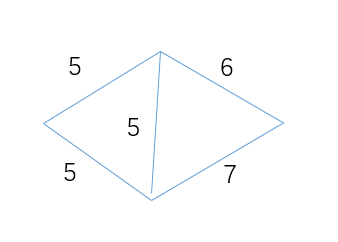
\includegraphics[width=0.4\linewidth]{11-1.png}\vspace{-10pt}
	\caption{the weighted graph} \nonumber\label{fig:the weighted graph}\vspace{-10pt}
\end{figure}
At the first step, there are 3 edges with weight 5, and there are 3 spanning of this multigraph.\\
\begin{figure}[H]
	\center
	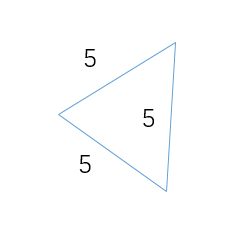
\includegraphics[width=0.4\linewidth]{11-2.png}\vspace{-10pt}
	\caption{the multigraph of edge with weight 5} \nonumber\label{fig:the weighted graph2}\vspace{-10pt}
\end{figure}
And we will add edge with weight 6. And we can get the spanning tree.\\
So we figure out that there are 3 minimum spanning tree.\\

\end{sol}

\end{document}
